\documentclass[a4paper,11pt]{report} 

\usepackage[utf8]{inputenc}
\usepackage[T1]{fontenc}
\usepackage{lmodern}
\usepackage[ngerman]{babel}

\usepackage{amsmath}
\usepackage{amssymb}
\usepackage{amsfonts}
\usepackage{amsthm}

\usepackage{subcaption}

\usepackage{graphicx}
\usepackage{xcolor}

\usepackage{tikz}
\usetikzlibrary{arrows,automata,calc,positioning}

\usepackage{blindtext}

\usepackage{listings}

% Farben
\usepackage{xcolor}

% Eclipse style colors
\definecolor{mygray}{rgb}{0.5,0.5,0.5}
\definecolor{myviolett}{HTML}{7F0055}
\definecolor{background}{HTML}{EEEEEE}

% lstlisting options
\lstset{%
	backgroundcolor=\color{background},
	basicstyle=\normalfont\ttfamily,
	breakatwhitespace=false,
	breaklines=true,
	captionpos=b,
	commentstyle=\color{mygray},
	escapeinside={\%*}{*)},
	extendedchars=true,
	frame=false,
	keepspaces=true,
	keywordstyle=\color{myviolett},
	language=c,
	numbers=left,
	numbersep=5pt,
	numberstyle=\tiny\color{mygray},
	rulecolor=\color{white},
	showspaces=false,
	showstringspaces=false,
	showtabs=false,
	stepnumber=1,
	stringstyle=\color{blue},
	tabsize=2,
}

\usepackage[%
hidelinks,
pdftitle={Systemnahes Programmieren},
pdfsubject={Dokumentation},
%pdfauthor={},
pdfkeywords={Systemnahes Programmieren, Compilerbau}
]{hyperref}

\addto\captionsngerman{\renewcommand{\chaptername}{Teil}}

\begin{document}

\begin{titlepage}
\centering
\vspace*{3cm}
{
\huge \scshape Systemnahes Programmieren
}
\par
\vspace*{2cm}
{
\huge Dokumentation
}
\par
\vspace*{4cm}
%vorgelegt von \\
%\vspace*{1cm}
{\huge Gruppe 35} \\
\vspace*{1cm}
{
\Large
\scshape
Kishor Rana, 43281 \\[1ex]
Jonas Weber, 43399 \\[1ex]
Tim Bierenbreier, 43235 \\[1ex]
Lutz Bader, 42887 \\
}
\vfill
Wintersemester 2016/2017 \\[1ex]
\today

\begin{tikzpicture}[remember picture,overlay]
%\draw[rounded corners=10pt] ($ (current page.north west) + (1,-1) $) rectangle ($ (current page.south east) + (-1,1) $);
\draw[rounded corners=20pt] ($ (current page.north west) + (1,-1) $) |- ($ (current page.south east) + (-1,1) $);
\draw[rounded corners=20pt] ($ (current page.north west) + (1,-1) $) -| ($ (current page.south east) + (-1,1) $);
\node[anchor=north east] at ($ (current page.north east) + (-2,-2) $) {
\includegraphics[width=.5\textwidth]{hska}};
\end{tikzpicture}

\end{titlepage}

\setcounter{page}{2}

\tableofcontents

\chapter{Lexikalische Analyse}

Ziel des Labors ist es, dass sich die Studierenden mit der Funktionsweise und der Implementierung eines Compilers vertraut machen.
Diese Funktionsweise lässt sich grob wie in der Abbildung \ref{fig:compiler} darstellen.

\begin{figure}
\centering
\begin{tikzpicture}[node distance = 3cm]
\node[rectangle,draw] (compiler) {Compiler};
\node (quelle) [left of = compiler] {Quellsprache};
\node (ziel) [right of = compiler] {Zielsprache};

\draw[->] (quelle) -- (compiler);
\draw[->] (compiler) -- (ziel);
\end{tikzpicture}
\caption{Schematische Darstellung eines Compilers}
\label{fig:compiler}
\end{figure}

Außerdem werden durch die Aufgabenstellung die Kenntnisse vieler Disziplinen vereint, da ein Compiler vielerlei Kenntnisse verlangt.
Die Aufgabe des Labors teilt sich grob in zwei Teile.
Zum einen soll im ersten Teil soll ein Scanner implementiert werden, der wiederum grundlegende Funktionen des Compilers beinhaltet.
Dieses ersten Kapitels der Dokumentation gibt einen Überblick über die grobe Implementierung des Scanners.

\section{Buffer}
Der Buffer dient als Zwischenspeicher für die eingelesene Datei.
Der Scanner bedient sich am Buffer, indem er aus ihm die Chars der eingelesenen Datei liest, wobei es die Aufgabe des Buffers ist, sich zur richtigen Zeit neu zu befüllen.
Die Klasse Buffer verwaltet zwei Objekte buffer1 und buffer2 vom Typ \texttt{BufferHalf}, sowie einen Pointer \texttt{bufferAktuell}, der auf die aktuell benutzte Bufferhälfte zeigt.
Eine Bufferhälfte besitzt ein Char-Array für die Speicherung der Zeichen, außerdem einen Counter, der die aktuelle Stelle im Buffer mitzählt, eine Variable \texttt{bytesread}, die die mit der Systemfunktion \texttt{read()} eingelesenen Bytes zählt und ein Flag \texttt{finished}, welches binär speichert, ob die Bufferhälfte fertig gelesen wurde.
Im Konstruktor \texttt{BufferHalf()} wird die Systemfunktion \texttt{posix\_memalign()} aufgerufen, um 1024 Byte für das Char-Array zu reservieren.
Ein char entspricht einem Byte, wodurch das Char-Array nun Indizes von 0 bis 1023 besitzt.
Im Konstruktor der Klasse Buffer werden zuerst zwei Objekte der Klasse \texttt{BufferHalf} erstellt.
Anschließend wird die Systemfunktion \texttt{open()} aufgerufen, der den Pfad der Datei übergeben wird, die zu öffnen ist.
Es wird ein Integer file descriptor zurückgegeben, der später der Systemfunktion \texttt{read()} übergeben werden muss, um die referenzierte Datei in den Buffer einzulesen.
Anschließend wird im Konstruktor noch dafür gesorgt, dass der Pointer \texttt{bufferAktuell} auf die erste Bufferhälfte buffer1 zeigt und der Spaltenzähler column und der Zeilenzähler line des Buffers auf 1 stehen.
Um den Buffer das erste Mal aufzufüllen, wird die Methode \texttt{fillBuffer()} aufgerufen.
Diese Methode ruft die Systemfunktion \texttt{read()} auf, welcher der oben genannte file descriptor übergeben wird, um die ersten 1024 Zeichen (Bytes) in das Char-Array der aktuellen Bufferhälfte einzulesen.
Die \texttt{read()}-Funktion liest immer ab der zuletzt gelesenen Stelle weiter.
Der Return-Wert der \texttt{read()}-Funktion ist die Anzahl der tatsächlich gelesenen Bytes (sind weniger als die geforderte Anzahl, falls die Datei vorher zu Ende ist) und wird in die Variable \texttt{bytesread} der aktuellen Bufferhälfte gespeichert.
Die Methode \texttt{getChar()} gibt das aktuelle Zeichen im Buffer zurück und zählt den Counter hoch.
Wenn das Ende der aktuellen Bufferhälfte erreicht ist, wird die Bufferhälfte ausgewechselt und die nächste aufgefüllt.
Wenn das Ende der eingelesenen Datei erreicht ist, wird \texttt{\#} zurückgegeben.
In \texttt{getChar()} wird des Weiteren jedes Mal die \texttt{column}-Variable der aktuellen Bufferhälfte hochgezählt, sowie die \texttt{line}-Variable, falls das aktuelle Zeichen ein Zeilenumbruch ist.
Wenn die aktuelle Bufferhälfte vollständig gelesen wurde, wird ihr \texttt{finished}-Flag gesetzt, das letzte Zeichen der Bufferhälfte wird zwischengespeichert, die Bufferhälften werden gewechselt, ihr Counter und ihr \texttt{finished}-Flag wird 0 gesetzt und die nun aktuelle Bufferhälfte wird mit der \texttt{read()}-Funktion neu befüllt.
Wenn das zwischengespeicherte letzte Zeichen der vorherigen Bufferhälfte der Nullterminator aus der gelesenen Datei ist (\texttt{\textbackslash n}) und das erste Zeichen der nächsten Bufferhälfte \texttt{\textbackslash 0} ist, also die Datei genau in die vorherige Bufferhälfte gepasst hat, wird \texttt{\#} zurückgegeben.
Wenn dies nicht der Fall ist, wird als nächstes das zwischengespeicherte Zeichen ausgegeben.
Ansonsten, wenn man sich in keinem Sonderfall befindet, wird ganz normal das aktuelle Zeichen der aktuellen Bufferhälfte ausgegeben.

\section{Automat}
Durch eine Zustandsübergangstabelle, die die gesamte Logik des Automaten beinhaltet, ist der Code überschaubar.
Er besteht insgesamt aus drei verschiedenen Teilen.
Abbildung \ref{fig:tabelle} zeigt die beschriebene Zustandsübergangstabelle im Detail.

\subsection{Die Zustandsübergangstabelle}
Der neue Zustand berechnet sich aus der Kombination aus dem aktuellen Zustand und der Eingabe.
Die Eingabe befindet sich in der Zustandsübergangstabelle in der ersten Spalte (Abbildung \ref{fig:tabelle_links}).
Der aktuelle Zustand ist in der ersten Zeile der Tabelle zu finden.
Die verschiedenen Kombinatinonsmöglichkeiten können dementsprechend zusammengesetzt werden.

Anfangs ist der Automat im Zustand 0.
Kommt ein Zeichen, welches getestet werden soll, zum Beispiel ein *, würde der Automat im Zustand 9 landen.
Da ein * ein fertiges Token ist, ist in der Spalte 9 des Automaten, egal bei welchem Input, der Zustand 109 eingetragen.
Alle "`Hunderter"'-Zustände sind in der Tabelle Endzustände, bei dem der Automat weiß, dass er ein bestimmtes Token ausgeben muss.

\begin{figure}[p!]
	\centering
	\begin{subfigure}[b]{.99\textwidth}
		\centering
		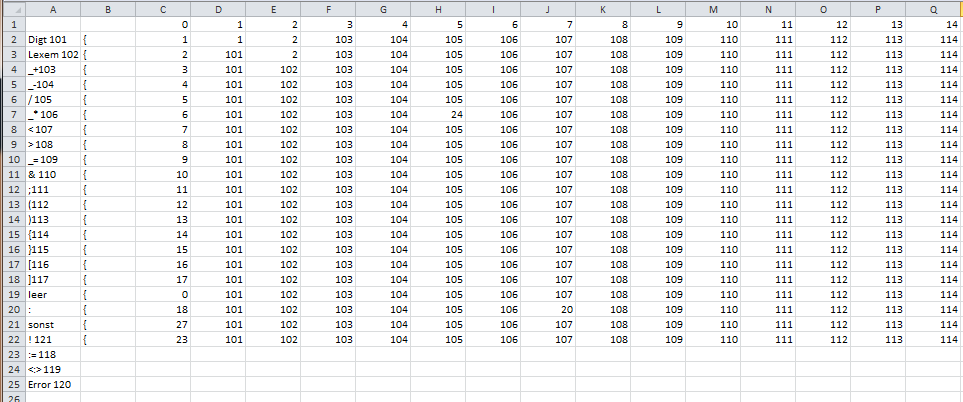
\includegraphics[width=.98\textwidth]{bilder/tabelle-links}
		\caption{Linke Hälfte der Übergangstabelle}
		\label{fig:tabelle_links}
	\end{subfigure}
	\par \bigskip
	\begin{subfigure}[b]{.99\textwidth}
		\centering
		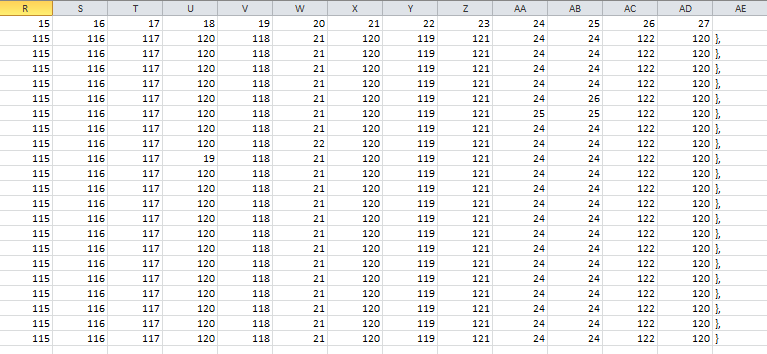
\includegraphics[width=.98\textwidth]{bilder/tabelle-rechts}
		\caption{Rechte Hälfte der Übergangstabelle}
		\label{fig:tabelle_rechts}
	\end{subfigure}
	\caption{Übergangstabelle}
	\label{fig:tabelle}
\end{figure}

\subsection{Eingabeumwandlung}
Hier werden die übergebenen Characters in die richtigen Integers umgewandelt, welche dann von der Zustandsübergangstabelle verarbeitet werden können.
Der zugehörige Quellcode ist in Listing \ref{lst:tabelle} in gekürzter Fassung zu finden.

\begin{lstlisting}[caption=Übergangstabelle, label=lst:tabelle]
int Automat::transformChar(char c) {
	int eingabe;

	if (c == '0' || // ...
	c == '9') eingabe = 0;
	else if (c == 'A' || // ...
	c == 'z') eingabe = 1;

	else if (c == '+') eingabe = 2;
	else if (c == '-') eingabe = 3;
	//...
	else if (c == ']') eingabe = 17;
	else if (c == ' ') eingabe = 18;
	else eingabe = 19;

	return eingabe;
}
\end{lstlisting}

\subsection{Der Check und die Ausgabe}
Hier werden zuerst der Eingabewert und der aktuelle Zustand in die Zustandsübergangstabelle gegeben.
Der neue Zustand wird anschließend zurückgegeben.
Jetzt wird anschließend gecheckt, ob es sich um einen Endzustand handelt oder nicht.
Ein Endzustand wäre, wie zuvor beschrieben, ein Zustand größer als Hundert.
Falls es ein Endzustand ist, wird der jeweilige Typ, also \texttt{TType}, des Tokens zurückgegeben und der aktuelle Zustand wieder auf 0 gesetzt.
Falls es sich nicht um einen Endzustand handelt, wird der \texttt{TType} \texttt{null} zurückgegeben.
Die einzige Ausnahme ist Zustand 21.
Dieser ist kein Endzustand, hat aber eine Ausgabe.
Dies wird benötigt, falls ein "`:"' auf ein "`<"' folgt, dann aber das Zeichen "`>"' ausbleibt.
Es muss auf das dritte Zeichen gewartet werden, damit eine Aussage zum \texttt{TType} getätigt werden kann.
Falls dieses ausbleibt, muss zuerst ein \texttt{TType} und dann ein \texttt{ErrorTType} ausgegeben werden, bevor weiter verfahren werden kann.
Ein Doppelpunkt darf somit nicht alleine stehen.
Was muss ich nun weiter beachten, wenn ich den Automat benutzen will?
Da der Automat nicht weiß, welches Zeichen als nächstes kommt, gibt er erst einen richtigen \texttt{TType} zurück, wenn ein Zeichen folgt, das nicht zu diesem Typ gehört.
Dieses Zeichen muss dann nochmal in den Automaten gegeben werden.
Falls man also einen \texttt{TType} ungleich Null zurück bekommt, muss man das Zeichen zuvor noch einmal testen lassen.
Falls Null zurück gegeben wird, kann der Automat mit dem nächsten Zeichen gespeist werden.
Dies ist zwar nicht sehr komfortabel, doch der Scanner weiß damit umzugehen.
Deshalb wäre hier eine Optimierung doppelt so viel Arbeit und wurde ausgespart.

\begin{lstlisting}[caption=Check und Ausgabe, label=lst:check]
TType Automat::checkChar(char c) {
	Automat::aktuellerZustand = zustandUebergangTabelle[Automat::transformChar(c)][aktuellerZustand];
	switch (Automat::aktuellerZustand) {
		case (eDigit): aktuellerZustand = anfang;
			return integer;
		case (eLexem): aktuellerZustand = anfang;
			return lexem;
		case (ePlus):  aktuellerZustand = anfang;
			return plusToken;
		// ...
		case (zUngleichFailed):
			return gleich;
		case (eError): aktuellerZustand = anfang;
			return error;
		case (eKommentar): aktuellerZustand = anfang;
			return kommentar;
		default:
			return null;
	}
}
\end{lstlisting}

\section{Symboltabelle}
Die Symboltabelle ist als \texttt{HashMap} umgesetzt.
Die wichtigsten Tokens werden mit der der Methode \texttt{initSymbols()} in die Symboltabelle eingetragen.
Die Symboltabelle dient dazu, die Tokens zu verwalten, zu denen Informationen wie das zugehörige Lexem und der zugehörige Wert gespeichert werden sollen.
Insbesondere trifft dies auf die Bezeichner zu.
Andererseits können auch einige in der Sprache vorhandenen Schlüsselwörter, wie beispielsweise \texttt{read} oder \texttt{print} in der Symboltabelle statt im Automaten verwaltet werden, was zu einer einfacheren Wartung des Automaten führt.
Bei der Umsetzung der Symboltabelle war ein wichtiger Eckpfeiler, dass sich Informationen schnell abrufen und einspeichern lassen.
Insofern haben wir uns dazu entschieden die Symboltabelle als \texttt{HashMap} zu implementieren.
Diese greift intern wiederum auf verkettete Listen zurück.

\subsection{HashMap}
Die \texttt{HashMap} für die Symboltabelle besteht aus \texttt{LinkedLists}, die Objekte vom Typ Token enthalten.
Die Methode \texttt{getTokenType(String lexem)} der \texttt{HashMap} nimmt als Argument ein Lexem (String) als Key entgegen, durchsucht die \texttt{HashMap} nach einem Token, bei dem dieser String übereinstimmt und gibt dann den \texttt{TType} des Tokens zurück.
\texttt{TType} ist als Enum verwirklicht, das alle möglichen \texttt{TokenTypes} definiert.
Durch einen Aufruf der Methode \texttt{insertToken(Token* t)} setzt ein Objekt vom Typ Token in die \texttt{HashMap} ein.
Für die Nutzung der \texttt{HashMap} wurden in die beteiligten Klassen Token und String passende \texttt{equals()} und \texttt{hashCode()} Methoden implementiert.

\subsection{LinkedList}
Die \texttt{HashMap} der Symboltabelle greift auf eine simple LinkedList-Implemen\-tier\-ung zurück.
Es handelt sich in diesem Fall um eine Klasse, die Token-Objekte speichern kann, die in Token-Node-Objekte verpackt sind.
Die To\-ken-Node-Objekte speichern jeweils eine Referenz auf das verpackte Token-Objekt und beinhalten zusätzlich Informationen zu dem vorherigen und folgenden Token-Node-Objekt in der Liste.
Somit wird die Funktionalität einer doppelt verketteten Liste umgesetzt, und das eigentliche Linked-List-Objekt speichert somit einfach nur auf das erste und letzte Token-Node-Element in der Liste.

\section{Scanner}
Der Scanner stellt sich als das Ziel der bis zu diesem Zeitpunkt entwickelten Unterkomponenten Buffer, Symboltabelle und Automat dar.
Insofern greift er auf diese zurück um aus einer gegebenen Datei Token für Token zu extrahieren und als Token-Objekt auszugeben.

Die Hauptmethode des Scanners heißt \texttt{nextToken()}.
Die Methode ist prinzipiell so aufgebaut, dass für jedes Zeichen, dass der Scanner vom Buffer holt zwei Phasen durchlaufen werden.

\begin{enumerate}
	\item Der Scanner cacht das aus dem Buffer entnommene Zeichen
	\item Der Automat prüft das Zeichen
	\begin{itemize}
		\item Falls noch nichts erkannt wurde, erweitert der Scanner seinen Lexem-String-Cache um das aufgenommene Zeichen und geht wieder in Phase 1
		\item Wenn der Automat das Zeichen direkt erkannt hat, wird es vom Scanner abgegeben
		\item Wenn ein Lexem erkannt wurde, das der Automat nicht direkt zuordnen kann, gibt der Scanner das Lexem an die Symboltabelle weiter
		\begin{itemize}
			\item Ist ein Eintrag in der Symboltabelle vorhanden, wird das passende Token mit der für das Lexem zugehörigen \texttt{Token\-In\-formation} vom Scanner rausgegeben.
			\item Ansonsten erstellt der Scanner ein neues Token mit dem Lexem. Zudem wird für das Lexem eine \texttt{TokenInformation} erstellt und wenn zutreffend wird auch der Zahlenwert des Tokens gespeichert.
			Das Token mit \texttt{TokenInformation} wird in der Symboltabelle eingetragen und der Scanner gibt dieses an den Methodenaufrufer zurück
		\end{itemize}
	\end{itemize}
\end{enumerate}

Sobald der Automat mittels des von uns verwendeten Stopzeichens \texttt{\#} dem Scanner signalisiert, dass das Ende der einzulesenden Datei erreicht worden ist, erstellt der Scanner ein Stop-Token.
Vom Automaten als fehlerhaft erkannte Tokens werden vom Scanner in einer Error-Message mit Zeile, Spalte und fehlerhaftem Zeichen ausgegeben.
Kommentare werden vom Automaten erkannt und der Scanner tauscht diese lediglich gegen Whitespace aus.

\chapter{Parser}
Zu Beginn ist in Abbildung \ref{fig:compiler} der grobe Ablauf eines Compilers dargestellt worden.
Die Abbildung \ref{fig:compiler_big} zeigt die einzelnen Schritte eines Compilers etwas mehr im Detail.
Dabei wird auch die Aufgabe eines Parsers innerhalb eines Compilers deutlich.
In der syntaktischen Analyse werden die Symbole des Quellprogramms zu einem Baum aufgebaut.
In der semantischen Analyse wird das Programm auf semantische Fehler geprüft, speziell die Korrektheit der Operanden.
Im letzten Schritt nach der Analyse wird die Zielsprache erzeugt.
In diesem Fall erfolgt die Übersetzung in die vorgegebene, an Assemblercode angelehnte Sprache, die vom mitgelieferten Interpreter ausgeführt werden kann.
Dieser Interpreter stellt darüber hinaus eine recht gute Hilfe zum Überprüfen der Ergebnisse dar.

\begin{figure}
\centering
\begin{tikzpicture}[node distance = 1.5cm, block/.style={rectangle,draw,minimum width=4cm}]
\node (quelle) {Quellsprache};

\node[block] (lex) [below of = quelle] {Lexikalische Analyse};
\node[block] (syntax) [below of = lex] {Syntaxanalyse};
\node[block] (sem) [below of = syntax] {Semantische Analyse};
\node[block] (code) [below of = sem] {Code-Generierung};

\node (ziel) [below of = code] {Zielsprache};

\draw[->] (lex) -- (syntax);
\draw[->] (syntax) -- (sem);
\draw[->] (sem) -- (code);

\draw[->] (quelle) -- (lex);
\draw[->] (code) -- (ziel);

\draw[thick] ($ (lex.north west)+(-0.25,0.25) $) rectangle ($ (code.south east)+(0.25,-0.25) $);

\draw[thick,dotted,red] ($ (syntax.north west)+(-0.5,0.5) $) rectangle ($ (code.south east)+(0.5,-0.5) $) node[below right] {Parser} ;

\end{tikzpicture}
\caption{Schritte eines Compilers}
\label{fig:compiler_big}
\end{figure}

In den folgenden Kapiteln soll nun die Implementierung des Parsers genauer erläutert werden.

\section{Parsing}
Im zweiten Teil der Aufgabe wird nun der Parser implementiert.
Der Parser bildet somit das abschließende Glied in der Kompilierung, allerdings steht der Parser noch vor der Code-Generierung.

Im ersten Schritt, dem sogenannten "`Parsing"', baut der Parser unter Zuhilfenahme des Scanners einen Baum aus einem gegebenen Quellcode auf.
Durch Verwendung dieses Baums können darauffolgend Code-Analyse Prozesse angestoßen werden.
Wir verwenden hierzu das Visitor-Pattern, das es uns erlaubt ein Visitor-Objekt durch den Baum zu schicken.
Maßgeblich sind der \texttt{TypeCheckVisitor}, der die Evaluierung beziehungsweise die Typisierung durchführt und der \texttt{CodeGeneratorVisitor}, der beim Durchlaufen des Quellcodes Assembler-Anweisungen generiert.
Ein oder mehrere Tokens finden sich nach dem Parsing als Knotenpunkte beziehungsweise Nodes in einer Baumhierarchie wieder.
Abbildung \ref{fig:uml} zeigt das zugehörige Klassendiagramm.

\begin{figure}
\centering

\tikzstyle{class}=[
    rectangle,
    draw=black,
    text centered,
    anchor=north,
    text=black,
    text width=3.25cm,
    minimum height=3cm
]

\begin{tikzpicture}[node distance=3cm]

\node[class, rectangle split, rectangle split parts=3] (parsetree) {\textbf{ParseTree} \nodepart{second} $\cdots$ \nodepart{third} + \texttt{parse()} \\ + \texttt{accept()} \\ $\cdots$ };


\node[class, rectangle split, rectangle split parts=2,anchor=north west] (node) [below of = parsetree] {\textbf{Node} \nodepart{second} \texttt{+childrenNodes} \\ \texttt{+rule}}; 
\node[class, rectangle split, rectangle split parts=2,anchor=north east] (leaf) [left=1cm of node] {\textbf{Leaf} \nodepart{second} \texttt{+token}}; 

\node[class, rectangle split, rectangle split parts=2] (statements) [below of = node] {\textbf{DeclsNode}}; 
\node[class, rectangle split, rectangle split parts=2] (decls) [left=.5cm of statements] {\textbf{StatementsNode}}; 
\node[class, rectangle split, rectangle split parts=2] (cdots) [right=.5cm of statements] {\textbf{$\cdots$} };

\draw[thick,->,arrows={-open triangle 45}] (leaf.north) -- ++(0,.5) -| ($ (parsetree.south west) + (.5,0)$);
\draw[thick,->,arrows={-open triangle 45}] (node.north) -- (parsetree);

\draw[thick,->,arrows={-open triangle 45}] (decls.north) -- ++(0,.25) -| ($ (node.south) - (.5,0)$);
\draw[thick,->,arrows={-open triangle 45}] (statements.north) -- (node.south);
\draw[thick,->,arrows={-open triangle 45}] (cdots.north) -- ++(0,.25) -| ($ (node.south) + (.5,0)$);

\end{tikzpicture}
\caption{Vereinfachtes UML}
\label{fig:uml}
\end{figure}

Die Baumhierarchie ergibt sich daraus, dass Nodes wieder Kinder oder ChildrenNodes haben.
Endpunkte oder Blätter im Baum sind vom Typ \texttt{Leaf}, haben keine Kinder (sie erben nicht von Nodes sondern dessen Basisklasse ParseTree) und ihnen lassen sich Tokens zuordnen.
Der Prozess des Parsings gestaltet sich implizit aus den Regeln der Grammatik, der zu implementierenden Sprache.
Ausgangspunkt für unseren Parser-Baum ist ein Knotenpunkt vom Typ \texttt{ProgramNode}, der wie sich aus der Grammatik zwingend ergibt ein \texttt{Decls-} und ein \texttt{Statement}-Node als Kinder haben muss.
Abbildung \ref{fig:baum} stellt den beschriebenen Sachverhalt grafisch dar.

\begin{figure}
\centering
\begin{tikzpicture}[->,>=stealth',shorten >=1pt,auto,node distance=2.5cm,semithick]
\tikzstyle{every state}=[rectangle, rounded corners,font=\ttfamily]

\node[state] (prog) {prog};
\node[state] (decls) [below left of = prog] {decls};
\node[state] (statements) [below right of = prog] {statements};

\node[state] (x) [below left of = decls] {\fbox{decl} \enskip \textcolor{red}{;} \enskip decls};
\node[state] (epsilon) [below right of = decls] {\normalfont $\varepsilon$};
\node[state] (cdots) [below right of = statements] {$\cdots$};

\node[state] (xx) [below of = x] {\textcolor{red}{int} \enskip \fbox{array} \enskip \textcolor{blue}{identifier}};

\node[state] (xxx) [below left of = xx] {\textcolor{red}{[} \enskip \textcolor{blue}{integer} \enskip \textcolor{red}{]}};
\node[state,anchor=north west] (epsilon2) [below right of = xx] {\normalfont $\varepsilon$};

\path
	(prog) edge (decls)
	(prog) edge (statements)
	(decls) edge (x)
	(decls) edge (epsilon)
	(statements) edge (cdots)
	($ (x.south) - (.75,-.2) $) edge (xx)
	($ (xx.south) - (.75,-.2) $) edge (xxx)
	($ (xx.south) - (.7,-.2) $) edge (epsilon2);
\end{tikzpicture}
\caption{Baum nach dem Schema der Grammatik}
\label{fig:baum}
\end{figure}

Der Parser delegiert das Parsing mittels der \texttt{parse()} Funktion an die Knotenpunkte im Baum weiter.
Wichtig ist, dass die \texttt{parse()}-Funktion jeweils einen Boolean zurückgibt, der Aussage darüber gibt, ob der Knoten-Punkt geparst werden konnte.
Die Knotenpunkte definieren je nach Typ (Prog, Decls, Statement, Decl, etc.) welche Knotenpunkte sie zum Parsen auffordern und gegebenenfalls bei Erfolg signalisierendem Rückgabewert aus der \texttt{parse()}-Methode als ihre Kinder hinzufügen.
Zudem wird beim Parsing in den Knoten im Feld \texttt{rule} eingespeichert nach welcher Regel ein neuer Teilbaum entsteht.
Betrachten wir beispielsweise das "`Statement"'-Symbol aus der Grammtik, so kann dieses nach sechs Regeln einen Teilbaum aufspannen.
Wird ein Endknotenpunkt beziehungsweise Leaf entsprechend des vom hinzufügenden Knoten erwarteten Tokentyps erfolgreich geparst, so gibt es dem Parser, durch Aufruf auf dem Parser der \texttt{nextToken()}-Funktion, dadurch Bescheid, dass ein neues Token vom Scanner angefordert wird.
Während sich der Baum implizit durch seine Knoten aufbauen lässt, sorgt dies dafür, dass die Leafs Token für Token den Quellcode verarbeiten.

\subsection{Visitor-Pattern}
Mithilfe des Visitor-Patterns kann der im vorherigen Schritt gebaute Baum für die Semantische Analyse und die Codegenerierung durchlaufen werden.
Beide Komponenten bedienen sich dem gleichen Prinzip, daher erben der TypeCheckVisitor und der CodeGenerationVisitor beide von derselben Superklasse (Abbildung \ref{fig:visitor}).
Durch dieses Patterns ist es möglich, die Operationen von den Knoten und Blättern selbst zu kapseln.
Die Superklasse Visitor setzt voraus, dass ihre erbenden Klassen hierfür die Besuchsfunktion visit implementieren müssen.
Selbstverständlich unterscheidet sich die Implementierung des jeweiligen abgeleiteten Visitors.
Der TypeCheckVisitor implementiert in seinen visit-Funktione die Logik für die Semantische Analyse und der CodeGeneratorVisitor implementiert die Logik für die Generierung des Maschinencodes der Zielsprache.

\begin{figure}
\centering
\begin{tikzpicture}[->,>=stealth',shorten >=0pt,auto,node distance=3cm,semithick]
\tikzstyle{every state}=[rectangle,minimum width=3cm,minimum height=2cm]

\node[state] (visitor) {Visitor};
\node[state,anchor=north west] (typecheck) [below left=1cm of visitor] {TypeCheckVisitor};
\node[state,anchor=north east] (codegenerator) [below right=1cm of visitor] {CodeGeneratorVisitor};

\draw[thick,->,arrows={-open triangle 45}] (typecheck.east) -- ++(1,0) -| ($ (visitor.south) - (.5,0) $);
\draw[thick,->,arrows={-open triangle 45}] (codegenerator.west) -- ++(-1,0) -| ($ (visitor.south) + (.5,0) $);
\end{tikzpicture}
\caption{Visitor}
\label{fig:visitor}
\end{figure}

\section{Semantische Analyse}
In der semantischen Analyse wird die Einhaltung der Regeln der Grammatik geprüft und im Fehlerfall ein entsprechender Fehler ausgegeben.
Die semantische Analyse wird vom \texttt{TypeCheckVisitor} implementiert.
Die Analyse des Baumes verläuft hierfür mithilfe des Visitor-Patterns nach dem Prinzip des rekursiven Abstiegs.
Durch diese Typisierung der Knoten des Baumes und der Blätter ist zum Beispiel es möglich, Fehler wie die Deklarierung eines Arrays mit Größe null aufzudecken.
Jeder Knoten und jedes Blatt speichert also genau einen Typ.
Die Besonderheit dabei ist, dass dieser Typ für die Blätter in der Symboltabelle hinterlegt wird.
Somit ist es beispielsweise möglich festzustellen, ob eine Identifier bereits deklariert wurde.

\section{Codegenerierung}
Die eigentliche Codegenerierung wird im letzten Schritt im \texttt{CodeGenerator\-Visitor} implementiert.
Hier wird ausgehend vom Baum und den gesetzten Typen seiner Knoten der Assemblercode entsprechend erzeugt und mit dem \texttt{FileWriter} in eine Datei geschrieben.

Zur Verdeutlichung der Codegenerierung soll das Listing \ref{lst:codegenerator} angeführt werden.
Der Quellcode ist gekürzt und soll nur die wesentliche Vorgehensweise aufzeigen.

\begin{lstlisting}[caption=Codegenerierung, label=lst:codegenerator]
void CodeGeneratorVisitor::visit(StatementNode &statementNode) {
	if (statementNode.rule == ASSIGN_RULE) {
		Leaf *identifierLeaf = (Leaf *) statementNode.getChildrenNodes()->get(0);
		statementNode.getChildrenNodes()->get(3)->accept(*this);
		fileWriter->write("\nLA $");
		fileWriter->write(identifierLeaf->token->lexem);
		statementNode.getChildrenNodes()->get(1)->accept(*this);
		fileWriter->write("\nSTR");
	} else if (statementNode.rule == WRITE_RULE) {
		// ...
	}
	//...
}
\end{lstlisting}

Eine erwähnenswerte Besonderheit liegt bei der Erzeugung von \texttt{if} beziehungsweise \texttt{else} Statements und dem \texttt{while} Statement.
Hier werden nämlich dynamische Sprungmarken erstellt, die nur einmal benutzt werden.
Im Falle eines \texttt{if} beziehungsweise \texttt{else} Statements werden zwei unterschiedliche Sprungmarken benötigt.
Dies wurde mithilfe einer Laufvariable realisiert, die für jede neue Sprungmarke erhöht wird und am Ende des \texttt{\#label} hinzugefügt.
Somit wird eine einzigartige Sprungmarke generiert.

\end{document}
